\documentclass{standalone}
\usepackage{tikz}
\usepackage{pgfplots}
\begin{document}
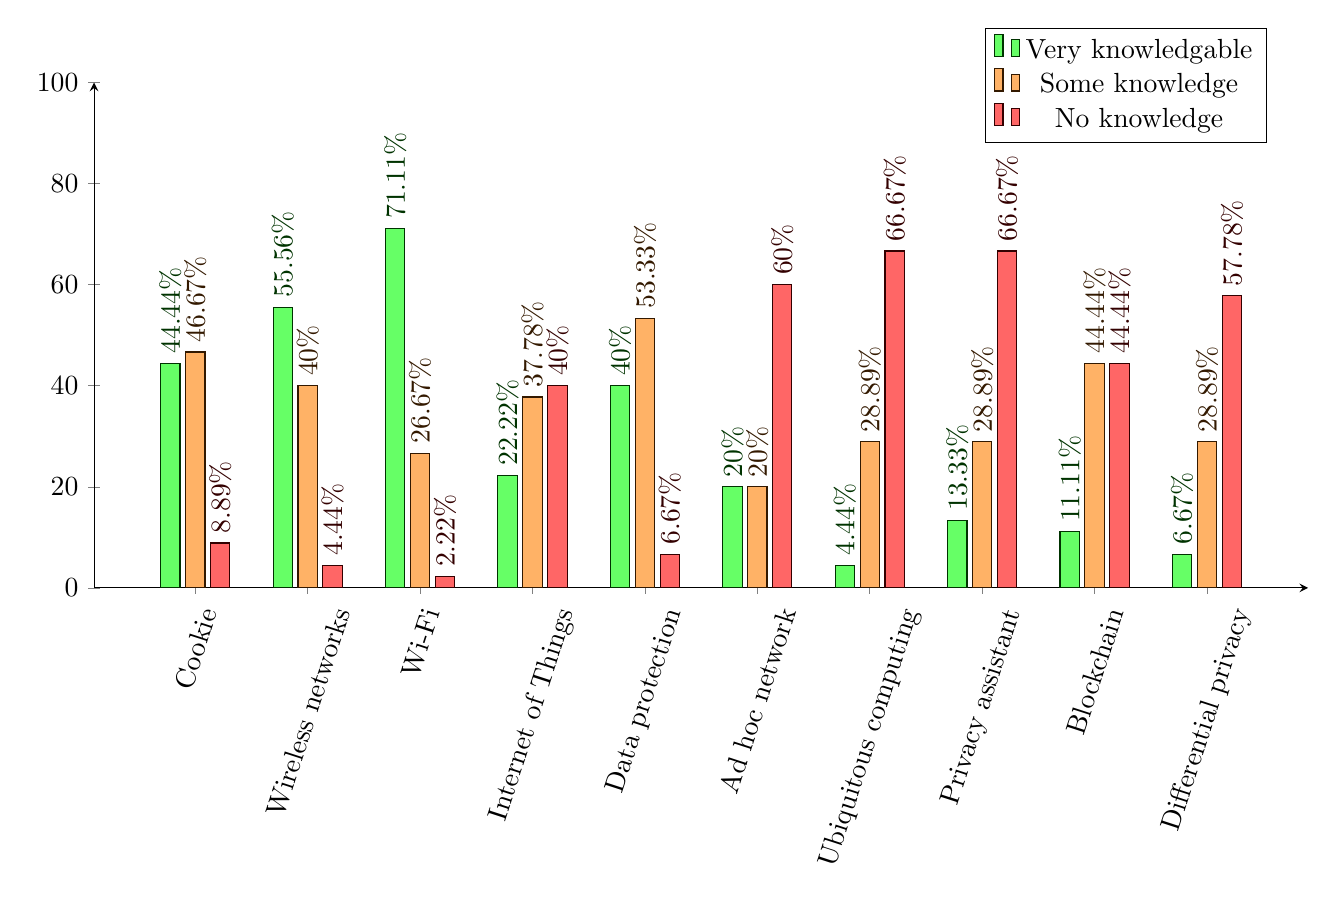
\begin{tikzpicture}
    \begin{axis}[
        height=8cm,
        width=17cm,
        symbolic x coords={Cookie, Wireless networks,Wi-Fi,Internet of Things,Data protection,Ad hoc network,Ubiquitous computing,Privacy assistant,Blockchain,Differential privacy},
        ybar,
        bar width=7pt,
        ymin=0,
        ymax=100,
        xticklabel style={rotate=72},
        axis x line=bottom,
        axis y line=left,
        enlarge x limits=0.1,
        nodes near coords={\pgfmathprintnumber\pgfplotspointmeta\%},
        every node near coord/.append style={rotate=90, anchor=west},
        legend style={at={(0.85,0.88)},anchor=south}
    ]
        \addplot[green!20!black,fill=green!60!white] coordinates {(Cookie,44.44) (Wireless networks,55.56) (Wi-Fi,71.11) (Internet of Things,22.22) (Data protection,40) (Ad hoc network,20) (Ubiquitous computing,4.44) (Privacy assistant,13.33) (Blockchain,11.11) (Differential privacy,6.67)};
        \addlegendentry{Very knowledgable}
        \addplot[orange!20!black,fill=orange!60!white] coordinates {(Cookie,46.67) (Wireless networks,40) (Wi-Fi,26.67) (Internet of Things,37.78) (Data protection,53.33) (Ad hoc network,20) (Ubiquitous computing,28.89) (Privacy assistant,28.89) (Blockchain,44.44) (Differential privacy,28.89)};
        \addlegendentry{Some knowledge}
        \addplot[red!20!black,fill=red!60!white] coordinates {(Cookie,8.89) (Wireless networks,4.44) (Wi-Fi,2.22) (Internet of Things,40) (Data protection,6.67) (Ad hoc network,60) (Ubiquitous computing,66.67) (Privacy assistant,66.67) (Blockchain,44.44) (Differential privacy,57.78)};
        \addlegendentry{No knowledge}
    \end{axis}
\end{tikzpicture}
\end{document}
